\section{Graph embeddings}
\subsection{}

\begin{frame}{\alert{Text}: sparse symbolic representation}

\begin{center}
	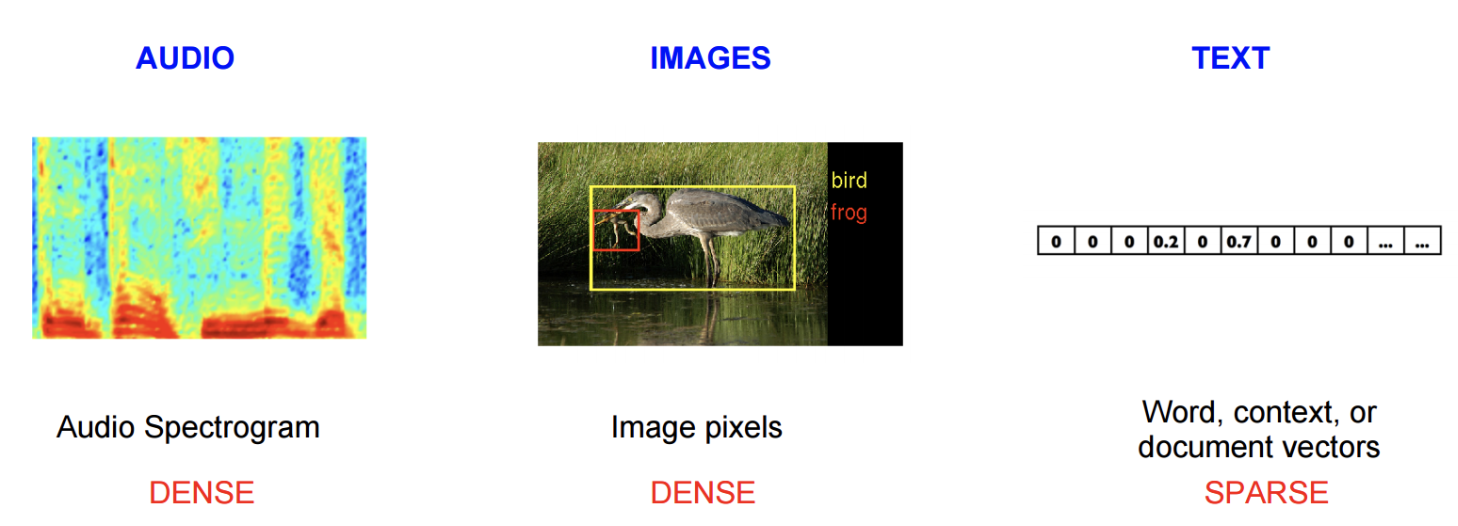
\includegraphics[width=\textwidth]{figures/w2v}
\end{center}

\pause 

Image source: \url{https://www.tensorflow.org/tutorials/word2vec}
	
\end{frame}




\begin{frame}{\alert{Graph}: sparse symbolic representation}

\begin{center}
	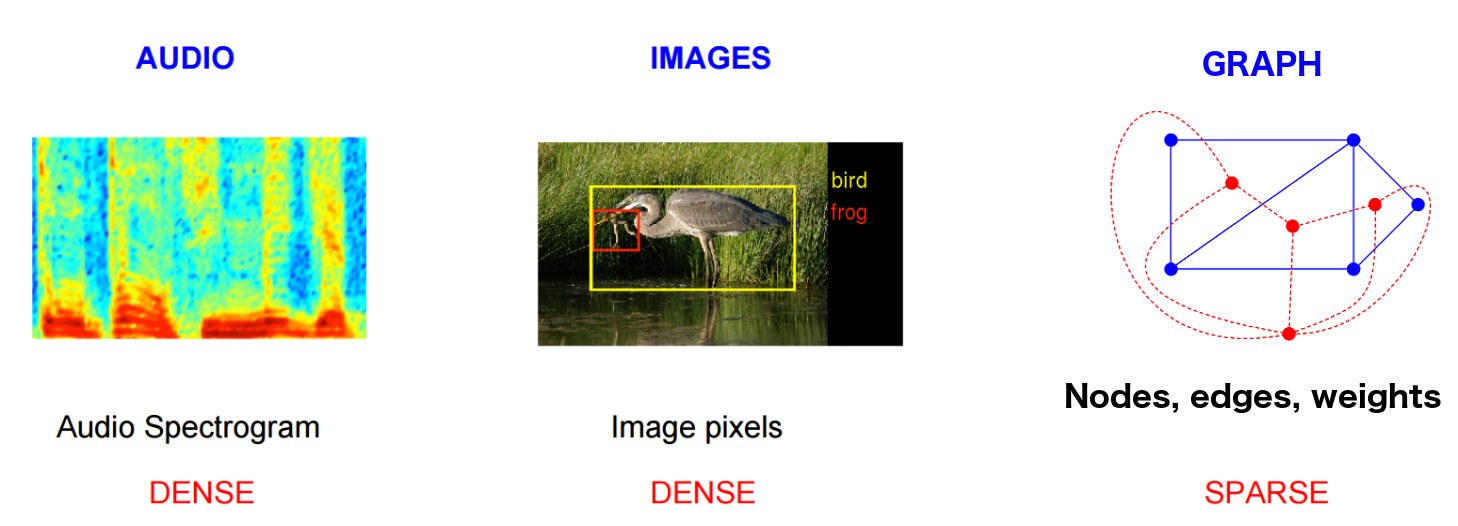
\includegraphics[width=\textwidth]{figures/g2v}
\end{center}
	
\end{frame}


\begin{frame}{Embedding graph into a vector space}

From a \textbf{survey on graph embeddings}~\cite{hamilton2017representation}:

\begin{center}
	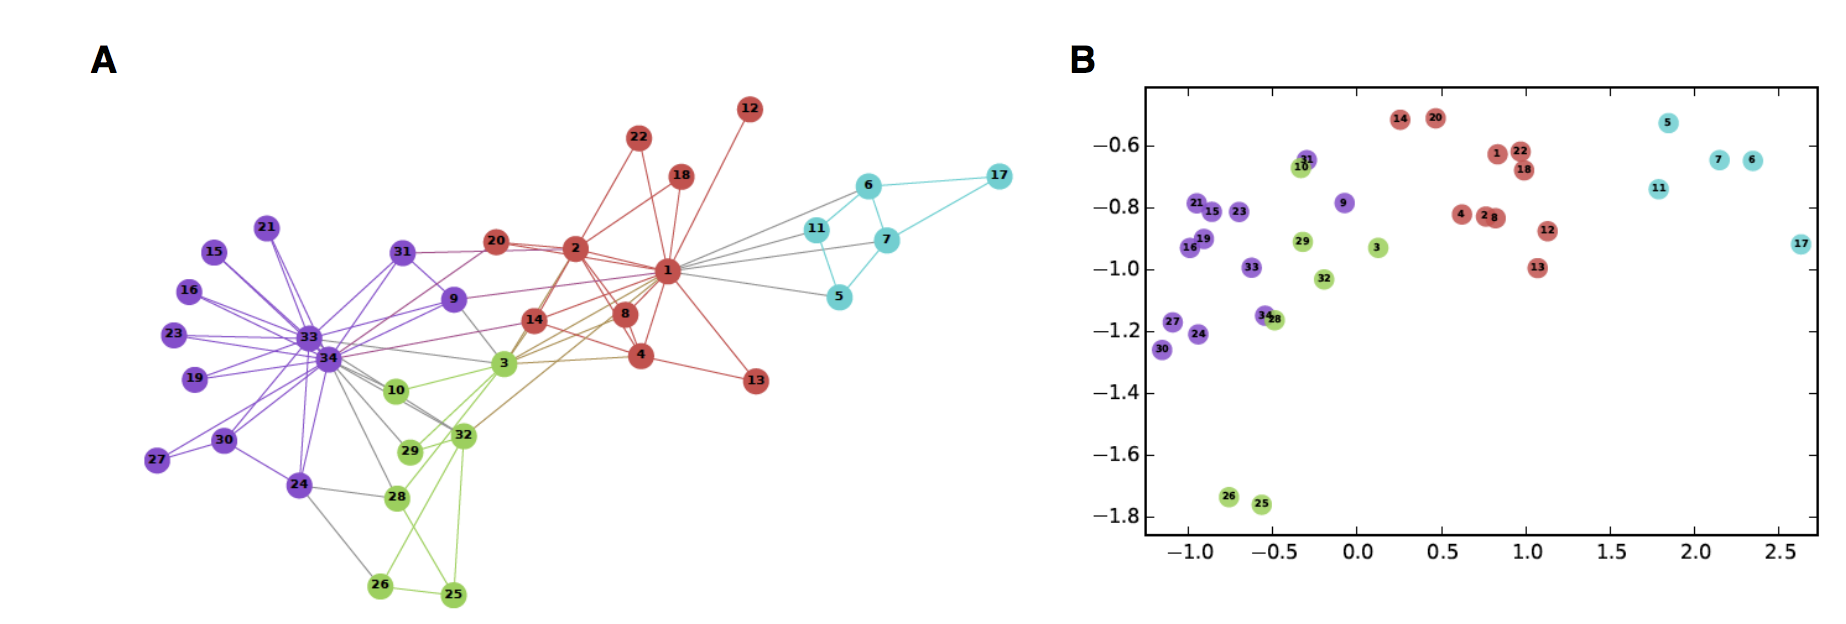
\includegraphics[width=\textwidth]{figures/ge-fig1}
\end{center}

	
\end{frame}



\begin{frame}{Learning with an ''autoencoder''}

From a \textbf{survey on graph embeddings}~\cite{hamilton2017representation}:

\begin{center}
	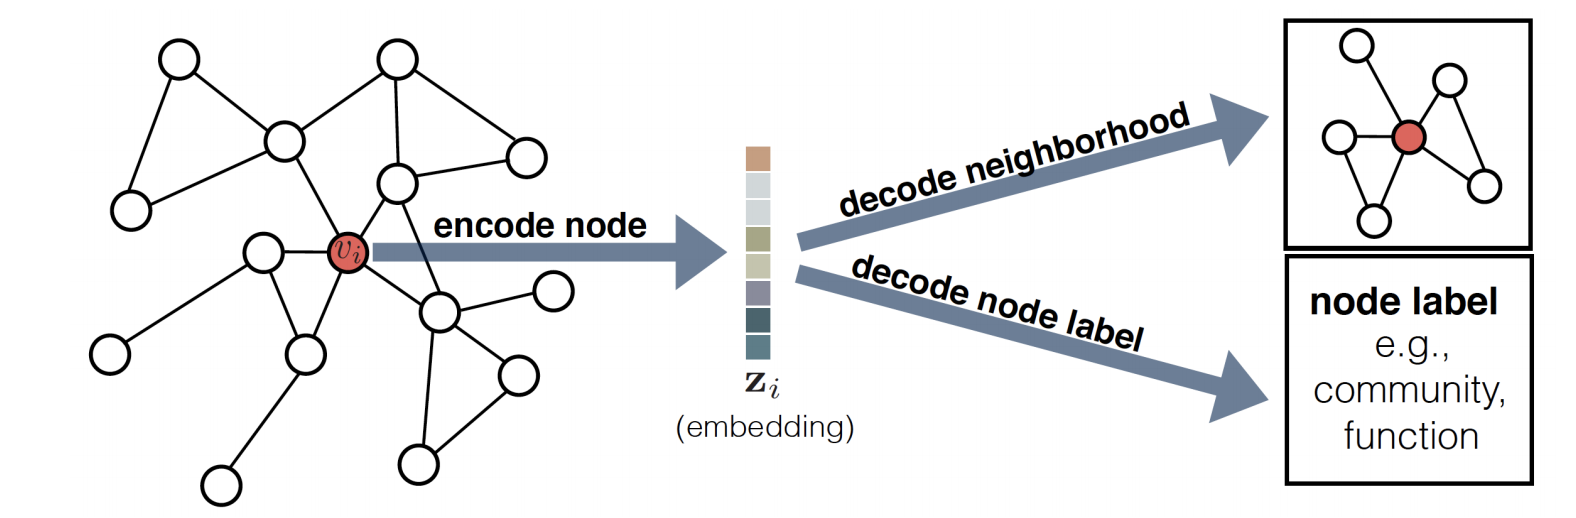
\includegraphics[width=\textwidth]{figures/ge-fig2}
\end{center}

	
\end{frame}




\begin{frame}{Some established approaches}

From a \textbf{survey on graph embeddings}~\cite{hamilton2017representation}:

\begin{center}
	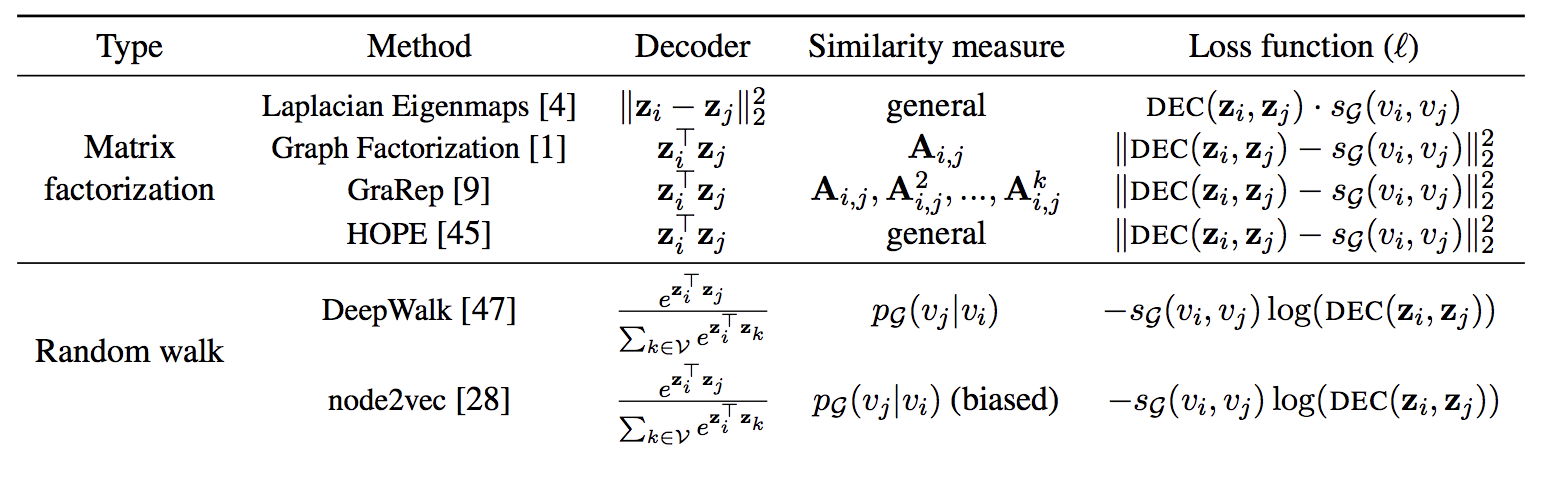
\includegraphics[width=\textwidth]{figures/ge-fig3}
\end{center}

	
\end{frame}





\begin{frame}{Graph embeddings using similarities}

%An submitted joint work with Andrei Kutuzov and Chris Biemann:


\begin{itemize}
\item Given a tree $(V, E)$

\item \alert{\textbf{Leackock-Chodorow (LCH)}} similarity measure:
$$
sim(v_i, v_j)= −\log\frac{shortest\_path\_distance(v_i, v_j) }{2h} 
$$

\pause 
\item \alert{\textbf{Jiang-Conrath (JCN)}} similarity measure:

$$
sim(v_i, v_j) = 2 \frac{\ln P_{\alert{lcs}}(v_i, v_j)}{\ln P(v_i) + \ln P(v_j)} 
$$
\end{itemize}
	
\end{frame}



\begin{frame}{Graph embeddings using similarities}

\textbf{path2vec} model (\url{arxiv.org/abs/1808.05611}): 

$$
\mathcal{L} = \frac{1}{|T|}  \sum_{ (v_i, v_j) \in T } \left( (\mathbf{v}_i^T \mathbf{v}_j - sim(v_i, v_j) )^2  + \alpha \mathbf{v}_i^T \mathbf{v}_{in} + \alpha \mathbf{v}_j^T \mathbf{v}_{jm} \right) ,
$$

%where:

\begin{itemize}
	\item $sim(v_i, v_j)$ - the value of a ''gold'' similarity measure between a pair of nodes $(v_i, v_j)$;
	\item $\mathbf{v}_i$ - an embeddings of node;
	\item $T$ - training batch; 
	\item $v_{in}$ - random adjacent node of $v_i$;
	\item $\alpha$ - a small regularization coefficient, e.g. $0.001$.
\end{itemize}



%
%$$
%J = \frac{1}{|T|}  \sum_{ (v_i, v_j) \in T }  (\mathbf{v}_i \cdot \mathbf{v}_j - sim(v_i, v_j) )^2,
%$$
%
%where:
%
%\begin{itemize}
%	\item $sim(v_i, v_j)$ - the value of a `gold' similarity measure between a pair of nodes $v_i$ and $v_j$;
%	\item $\mathbf{v}_i$ - an embeddings of node;
%	\item $T$ - training batch.
%\end{itemize}

\end{frame}

\begin{frame}{Speedup: graph vs embeddings}	

Computation of 82,115 pairwise similarities:

\begin{table}
\begin{tabular}{lc}
\toprule
\textit{Model} & \textit{Running time} \\
\midrule
LCH in NLTK & 30 sec. \\
JCN in NLTK & 6.7 sec. \\
%\midrule
FSE embeddings & 0.713 sec. \\
%\midrule
\textit{path2vec} and other float vectors & \textbf{0.007} sec. \\
\bottomrule
\end{tabular}
\end{table}

\end{frame}


\begin{frame}{Results: goodness of fit}


\textbf{Spearman correlation scores with WordNet similarities on SimLex999 noun pairs}:

\begin{table}
\begin{tabular}{lccc}
\toprule
& \multicolumn{3}{c}{\textit{Selection of synsets}} \\
Model & JCN-SemCor & JCN-Brown & LCH \\
\midrule
WordNet & 1.0  & 1.0  & 1.0  \\
\midrule
Node2vec & 0.655 & 0.671 & 0.724  \\
Deepwalk & 0.775 & 0.774  & 0.868 \\
FSE & 0.830  & 0.820 & 0.900  \\
\midrule
path2vec & \textbf{0.917}  & \textbf{0.914}  & \textbf{0.934}  \\
\bottomrule
\end{tabular}
\end{table}

\end{frame}




\begin{frame}{Results: SimLex999 dataset}


\textbf{Spearman correlations with human SimLex999 noun similarities:}


\begin{table}
\begin{tabular}{lc}
\toprule
\textit{Model} & \textit{Correlation} \\
\midrule
Raw WordNet JCN-SemCor & 0.487  \\
Raw WordNet JCN-Brown & 0.495  \\
Raw WordNet LCH & 0.513  \\
\midrule
node2vec { \cite{grover2016node2vec}} & 0.450  \\
Deepwalk { \cite{perozzi2014deepwalk}} & 0.533  \\
FSE { \cite{subercaze:2015}} & \textbf{0.556}  \\
path2vec JCN-SemCor & 0.549  \\
path2vec JCN-Brown & 0.540  \\
path2vec LCH & 0.540  \\
\bottomrule
\end{tabular}
\end{table}

\end{frame}



\begin{frame}{Results: SimLex999 dataset}

%\textbf{path2vec JCN-SemCor (no regularizers)}

\begin{figure}
    \centering
    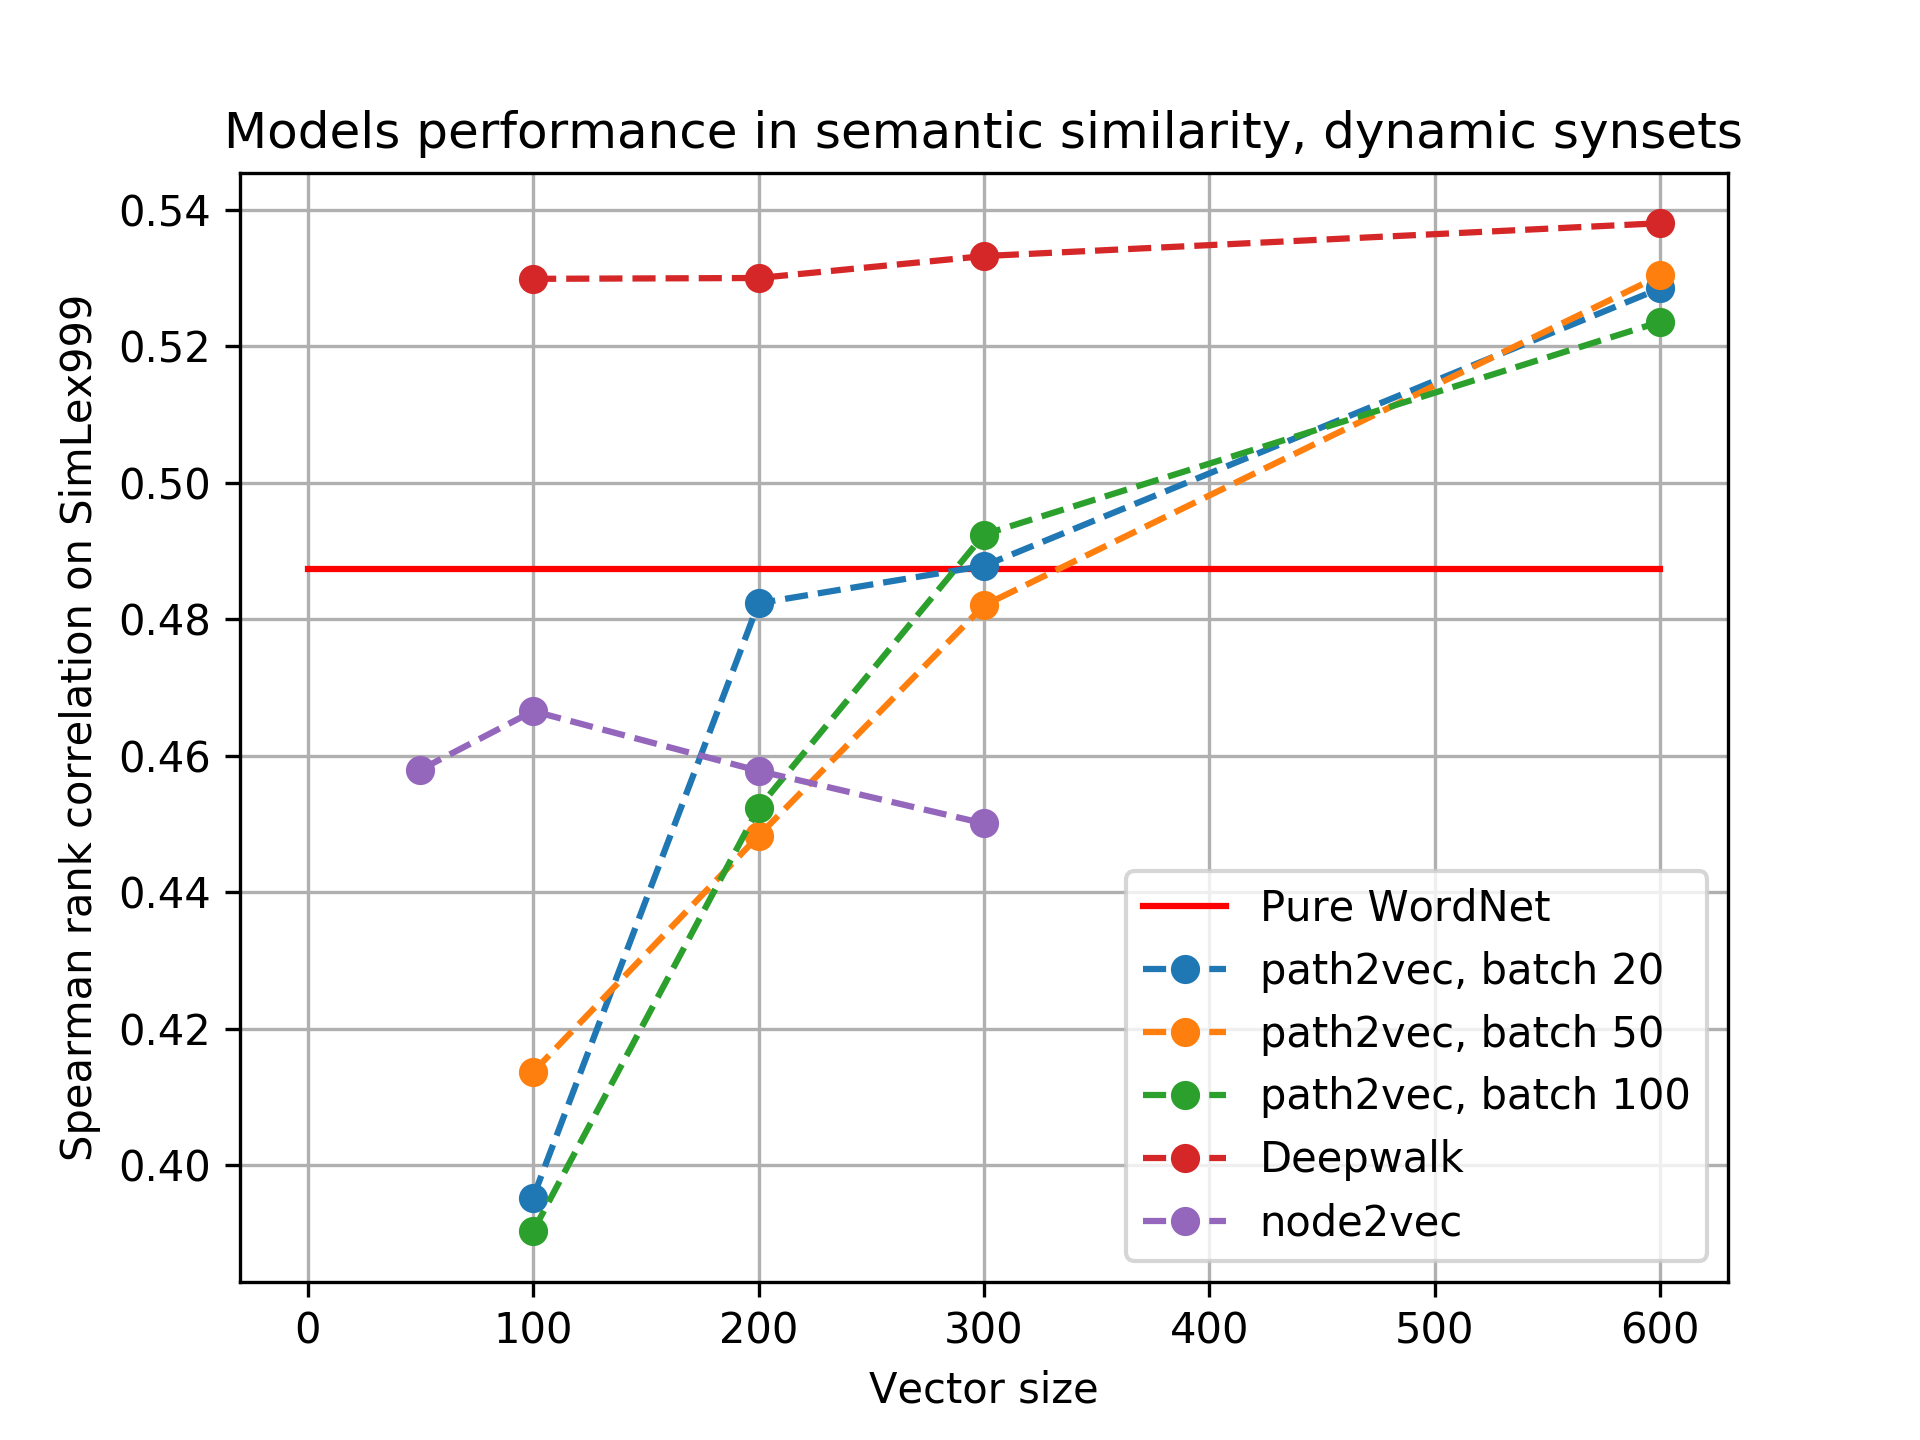
\includegraphics[width=0.79\textwidth]{figures/jcn-semcor-thresh01-near50_dynamic_synsets.png}
%     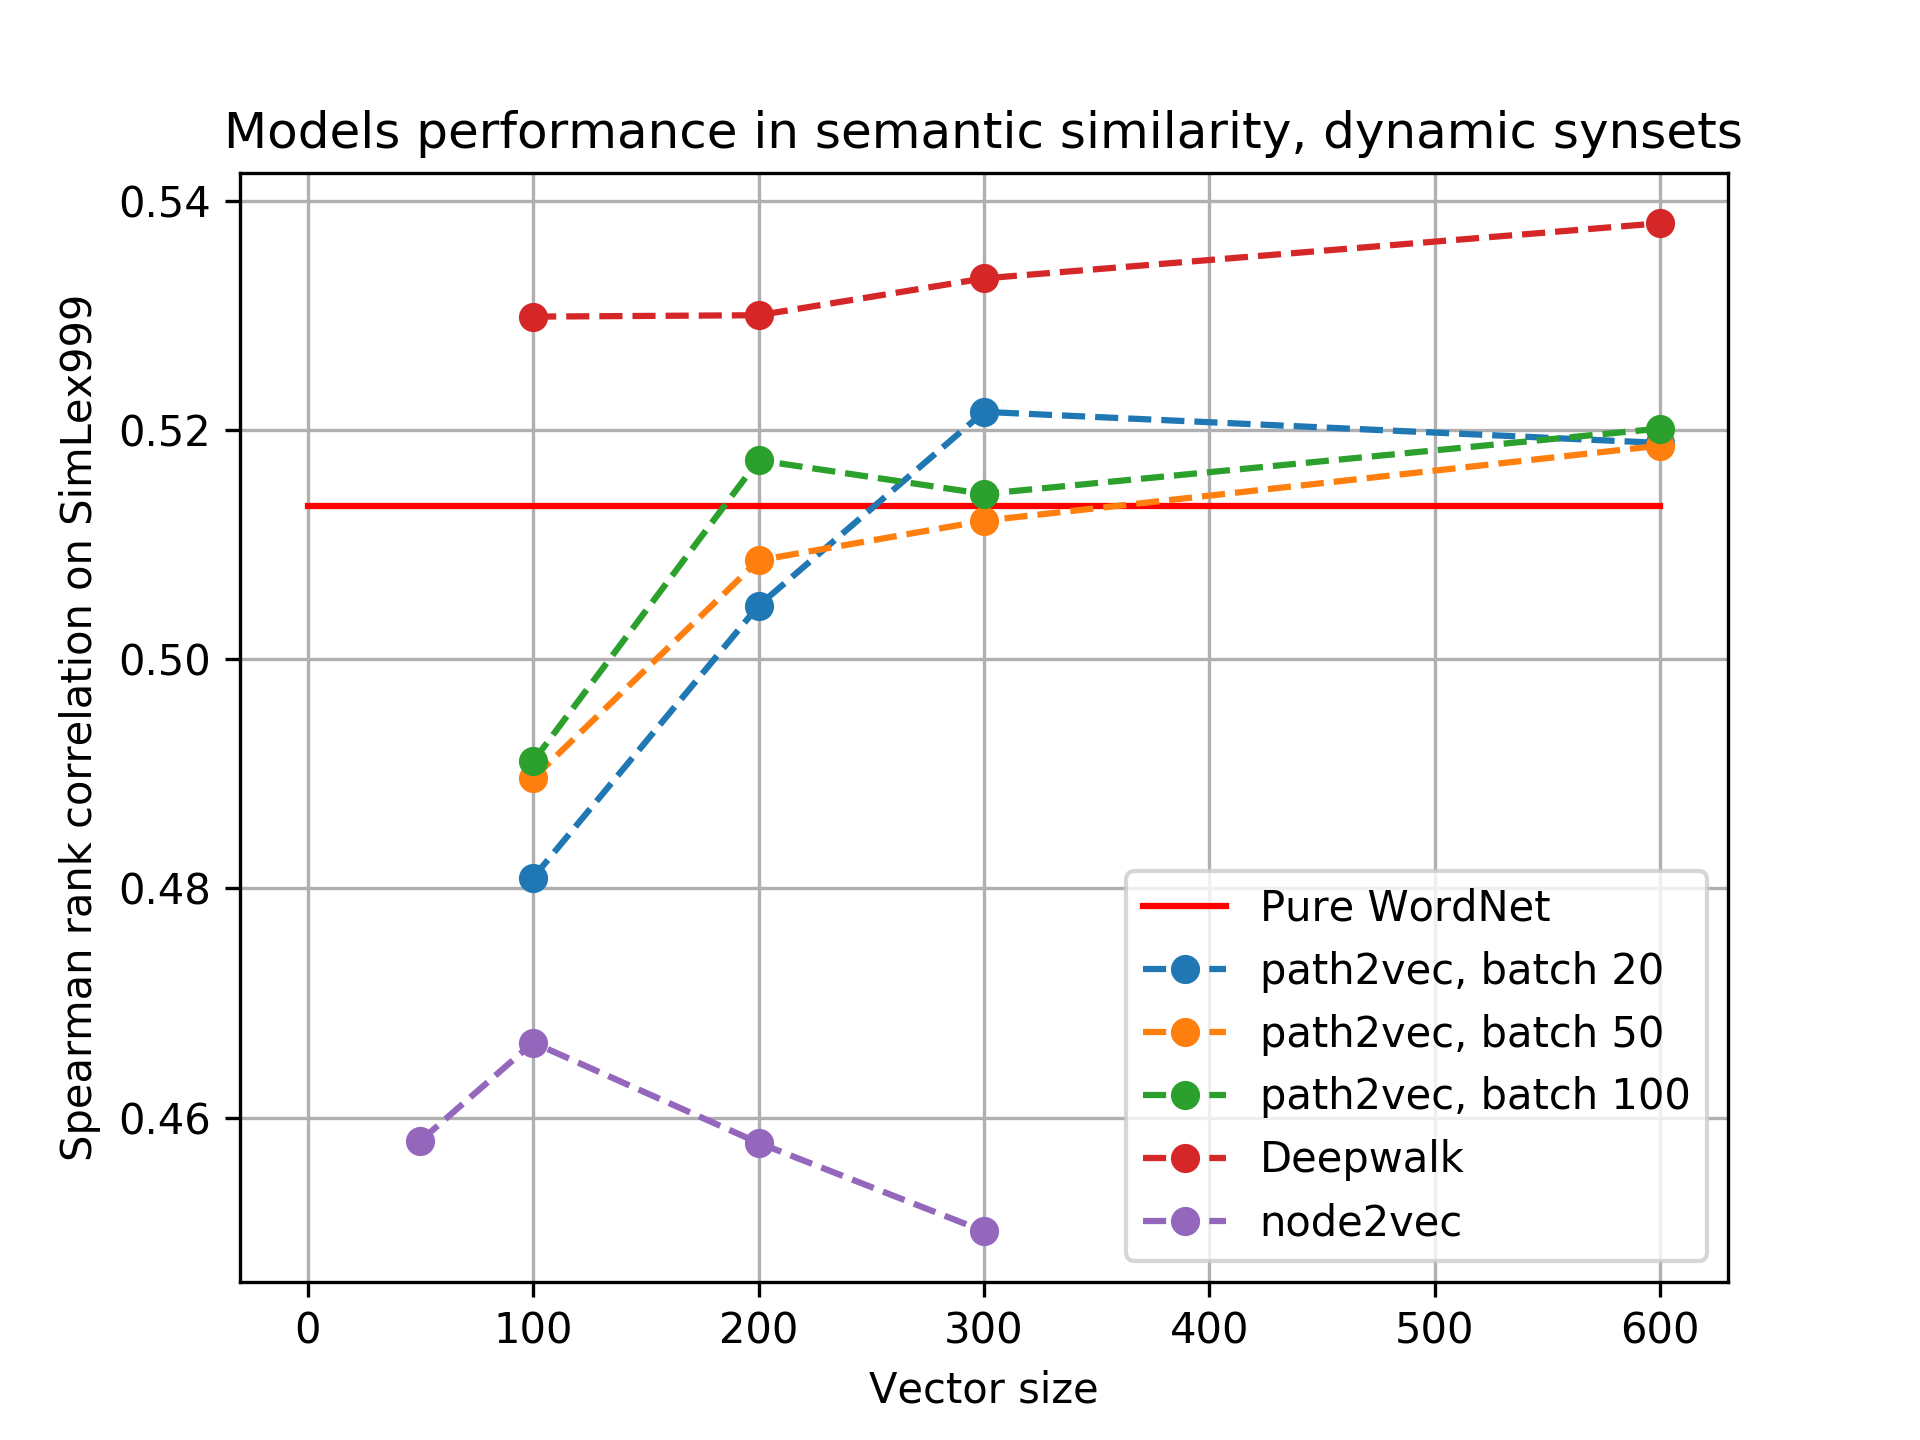
\includegraphics[width=0.49\textwidth]{figures/lch-thresh15-near50_dynamic_synsets.png}
       
\end{figure}
	
\end{frame}

%
%\begin{frame}{Results: word sense disambiguation}
%
%\textbf{WSD: each column lists all the possible synsets for the corresponding word.}
%
%
%\begin{figure}
%       \centering
%       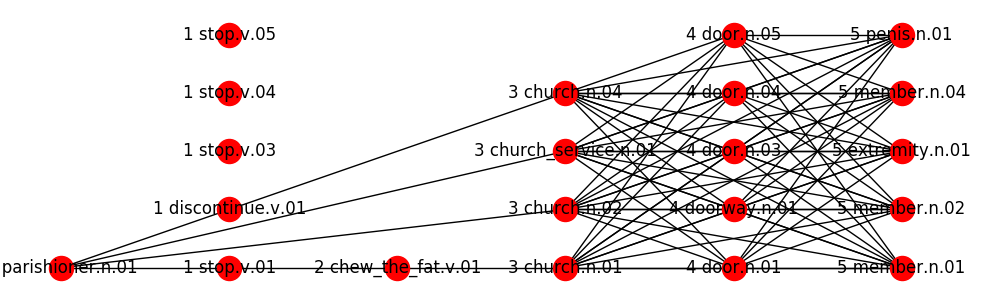
\includegraphics[width=\textwidth]{figures/graph_wsd_example}
%\end{figure}
%	
%\end{frame}
%

%\begin{frame}{Results: word sense disambiguation}
%
%\textbf{F1 scores on Senseval-2 word sense disambiguation task}:
%
%\begin{table}
%\footnotesize
%\begin{tabular}{lccc}
%\toprule
%Model & \multicolumn{3}{c}{F-measure} \\
%\midrule
%WordNet JCN-SemCor & \multicolumn{3}{c}{\textbf{0.620}} \\
%WordNet JCN-Brown &   \multicolumn{3}{c}{0.561} \\
%WordNet LCH & \multicolumn{3}{c}{0.547} \\
%node2vec~\cite{grover2016node2vec} & \multicolumn{3}{c}{0.501} \\
%Deepwalk~\cite{perozzi2014deepwalk} & \multicolumn{3}{c}{0.528} \\
%FSE~\cite{subercaze:2015}  & \multicolumn{3}{c}{0.536} \\
%\midrule
%\multicolumn{4}{c}{ \textit{path2vec}} \\
%\midrule
%\textit{Batch size:} & 20 & 50 & 100 \\
%\midrule
%JCN-SemCor & \textbf{0.543} & \textbf{0.543} & 0.535 \\
%JCN-Brown & 0.538 & 0.515 & 0.542 \\
%LCH & 0.540 & 0.535 & 0.536 \\
%\bottomrule
%\end{tabular}
%\end{table}
%	
%\end{frame}



%
%\begin{frame}{Improved Model and Results}
%
%%
%%Original model:
%%$$
%%\mathcal{L} = \frac{1}{|T|}  \sum_{ (v_i, v_j) \in T }  (\mathbf{v}_i \cdot \mathbf{v}_j - sim(v_i, v_j) )^2,
%%$$
%%
%%
%%Improved model:
%$$
%\mathcal{L} = \frac{1}{|T|}  \sum_{ (v_i, v_j) \in T } \left( (\mathbf{v}_i^T \mathbf{v}_j - sim(v_i, v_j) )^2  + \alpha \mathbf{v}_i^T \mathbf{v}_{in} + \alpha \mathbf{v}_j^T \mathbf{v}_{jm} \right) ,
%$$
%
%
%where:
%
%\begin{itemize}
%	\item $sim(v_i, v_j)$ - the value of a `gold' similarity measure between a pair of nodes $v_i$ and $v_j$;
%	\item $\mathbf{v}_i$ - an embeddings of node;
%	\item $T$ - training batch; 
%	\item $v_{in}$ - random adjacent node of $v_i$;
%	\item $\alpha$ - a small regularization coefficient, e.g. $0.001$.
%\end{itemize}
%
%\end{frame}
%
%
